\chapter{Resultados y Evaluación}
\label{cap:ResultadosYEvaluacion}

% (TODO) Texto introductorio
En este capítulo se muestran las pruebas realizadas sobre el prototipo 5 (\ref{cap:ArquitecturaFinal}).

\section{Definición de los Pipelines Experimentales}


% (ToDO) Texto descriptivo del diagrama de los pipelines
Como se explicó en el capítulo sobre la arquitectura final (\ref{cap:ArquitecturaFinal}), el prototipo 5 consta de varias posibles arquitecturas y funciones de pérdida, que se pueden combinar dando lugar a seis diferentes configuracinones (o \textit{Pipelines}). El diagrama \ref{fig:pipelines} muestra las diferentes topologías que se dan. Las arquitecturas y funciones de pérdida están ordenadas de tal manera que arriba a la izquierda se encuentra la configuración más simple (de la que se esperan los peores resultados) y abajo a la derecha la más compleja (la más prometedora). 

Con la evaluación y comparación de las diferentes configuraciones, se espera determinar cúal de ellas será la "definitiva", la que ofrezca mejores predicciones, pero teniendo también en cuenta sus tiempos de entrenamiento y la eficiencia general de las mismas. 

\begin{figure} 
    \centering
    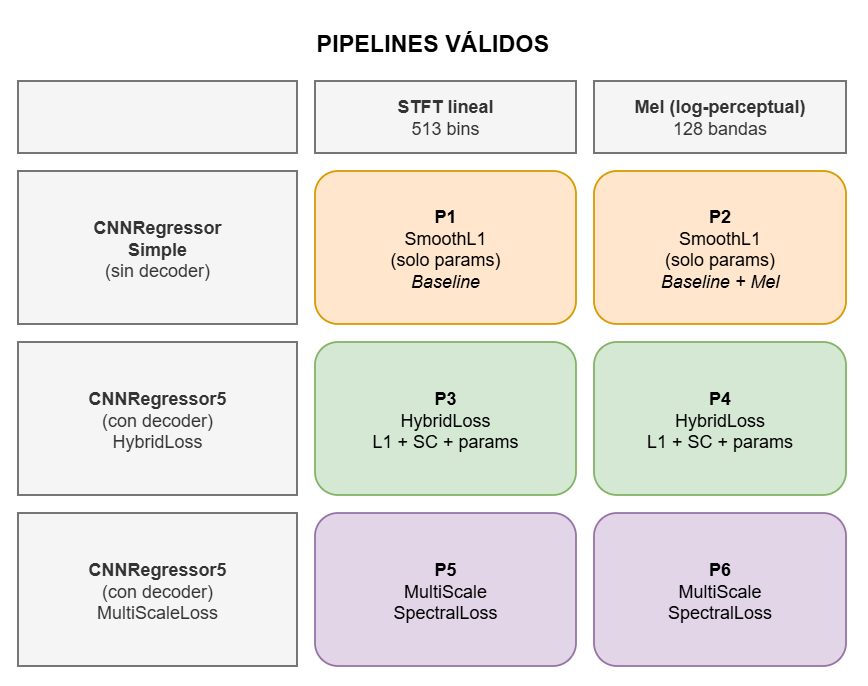
\includegraphics[width=1\textwidth]{Imagenes/Bitmap/pipelines}
    \caption{Representación de las diferentes combinaciones de Arquitecturas y Funciones de Pérdida.}
    \label{fig:pipelines}
\end{figure}

\section{Evaluación de las Diferentes Arquitecturas y Funciones de Pérdida}
La evaluación de las diferentes topologías se ha llevado a cabo con un único dataset de 50000 audios (método de generación explicado aquí: \ref{sec:gen_dataset}), un número que ha resultado ser equilibrado, perimitiendo unos resultados decentes sin suponer un incremento demasiado grande en los tiempos de entrenamiento de los modelos. 

El número de épocas no se ha dejado fijo, se ha utilizado un valor de paciencia (\textit{Early Stopping}) de 10 épocas. De esta manera, se comprueba el error de validación en cada época y si despues de 10 seguidas no se ha mejorado su record histórico, la red deja de entrenarse. Así pues, se evita la Sobreadaptación (\textit{Overfitting}) de la red neuronal, puesto que se evita un entrenamiento excesivo, y se ahorra tiempo de entrenamiento innecesario. 

Por otro lado, se ha elegido un \textit{Batch Size} de 32. Este, aparte de ser un estándar, es un valor asumible por cualquier tarjeta gráfica moderna y que consigue una eficiencia adecuada. 

\noindent \textbf{\textit{Benchmark}:}
\begin{itemize}
    \item \textbf{Tamaño del Dataset: 50000} 
    \item \textbf{Valor de Paciencia: 10} 
    \item \textbf{\textit{Batch Size}: 32} 
\end{itemize}

\subsection{P1: CNNRegressorSimple: SmoothL1, STFT lineal}

\subsubsection{Evaluación Mediante \textit{Test Set}}

\subsubsection{Evaluación Mediante \textit{Benchmark} Diverso}

\subsection{P2: CNNRegressorSimple: SmoothL1, Mel (log-perceptual)}

\subsubsection{Evaluación Mediante \textit{Test Set}}

\subsubsection{Evaluación Mediante \textit{Benchmark} Diverso}

\begin{figure} 
    \centering
    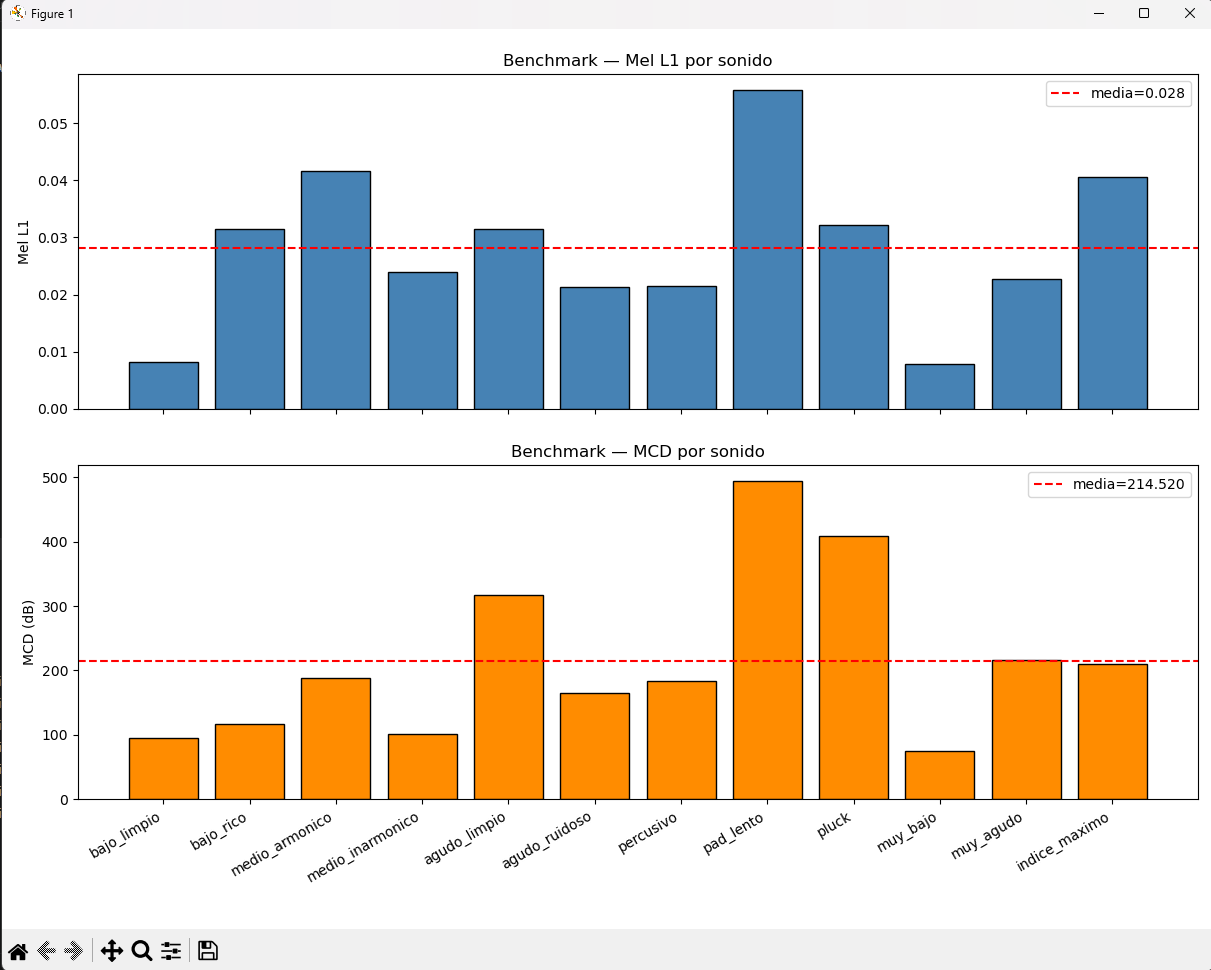
\includegraphics[width=1\textwidth]{Imagenes/Bitmap/benchmark_P2}
    \caption{Gráfico obtenido en la evaluación de P2 mediante \textit{benchmark}.}
    \label{fig:benchmarkP2}
\end{figure}

\begin{figure} 
    \centering
    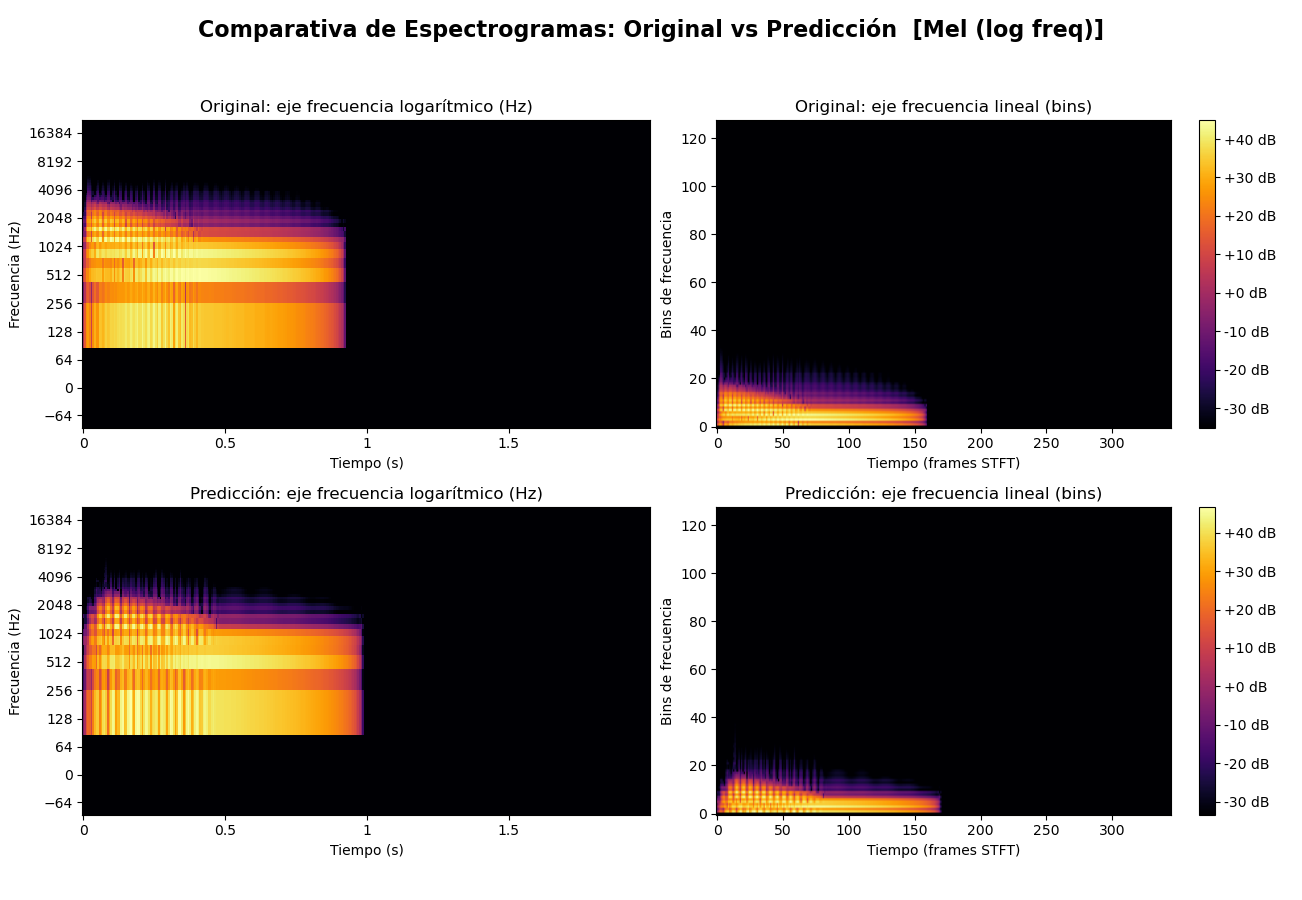
\includegraphics[width=1\textwidth]{Imagenes/Bitmap/espectrogramas_muy_bajo_P2}
    \caption{Espectrograma resultado de la predicción del audio de Benchmark: \textit{muy\_bajo}.}
    \label{fig:esp_muy_bajo_P2}
\end{figure}

\begin{figure} 
    \centering
    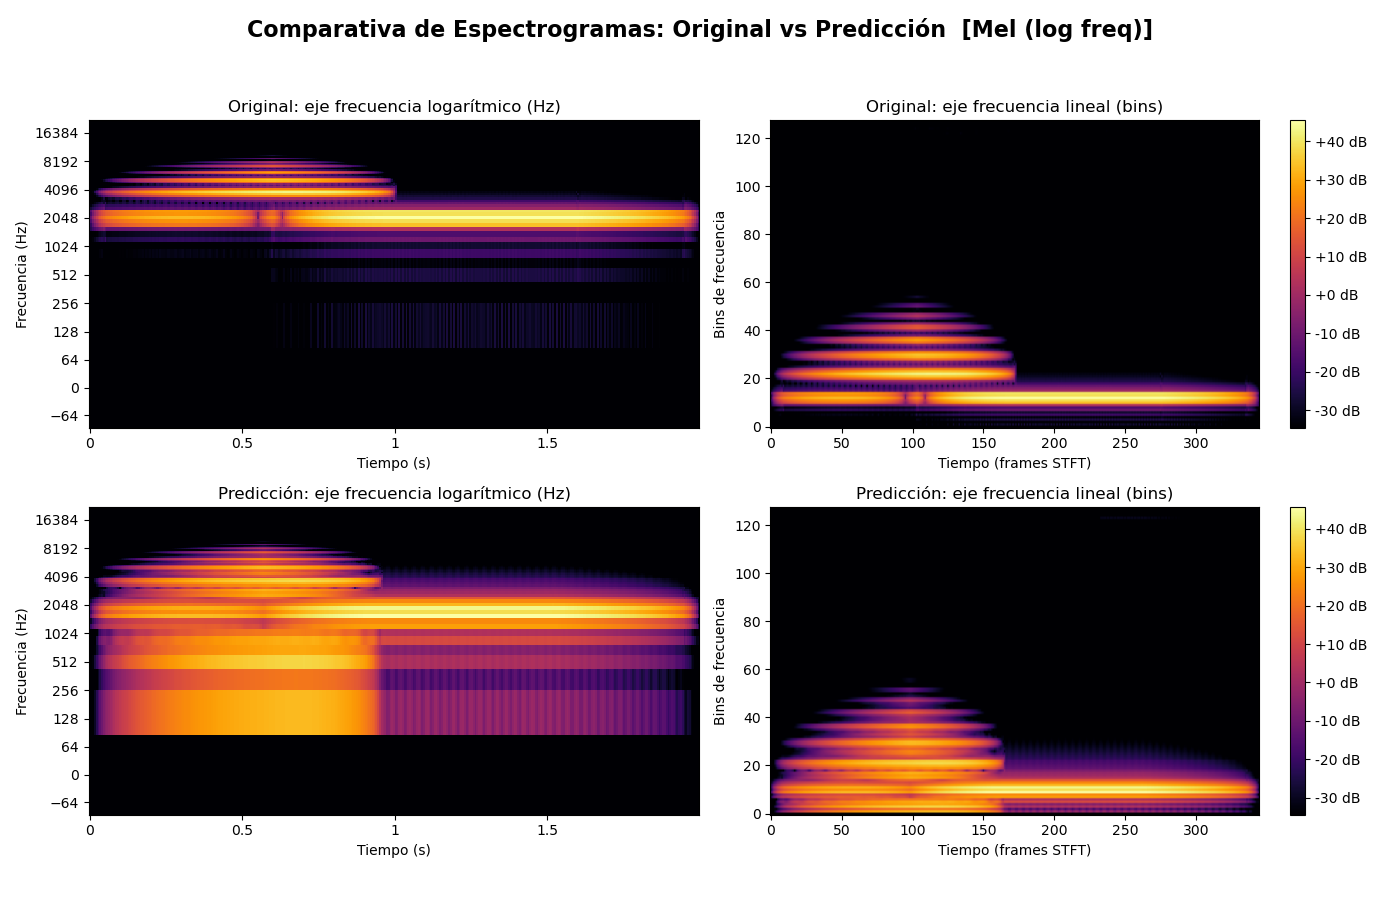
\includegraphics[width=1\textwidth]{Imagenes/Bitmap/espectrograma_pad_lento_P2}
    \caption{Espectrograma resultado de la predicción del audio de Benchmark: \textit{muy\_bajo}.}
    \label{fig:esp_pad_lento_P2}
\end{figure}

Al aplicar \textit{Mel L1} y \textit{MCD} sobre los resultados del \textit{benchmark}, obtenemos el gráfico \ref{fig:benchmarkP2}. A simple vista se puede apreciar que hay dos casos en los que las métricas, previamente mencionadas, se encuentran muy reducidas, estos casos son con el sonido \textit{bajo\_limpio} y con \textit{muy\_bajo}. Esto se debe a que las frecuencias bajas y limpias poseen patrones visuales muy claros y fáciles de asimilar para la red. Esto se puede ver, por ejemplo, en el espectrograma de \textit{muy\_bajo} y en el de la predicción de la red \ref{fig:esp_muy_bajo_P2}, en los que se aprecia su claridad y la similitud entre el original y la predicción.  

En contraposición, se hayan los resultados sobre el audio \textit{pad\_lento}, que destaca por haber generado un incremento de ambas métricas. Un \textit{pad} es un sonido de sintetizador caracterizado por comenzar muy lento (ataque bajo) y mantenerse. Comparando el espectrograma original de \textit{pad\_lento} y el de la predicción podemos sacar algunas conclusiones de estos resultados. Como se ve en la figura \ref{fig:esp_pad_lento_P2}, la red ha conseguido inferir perfectamente los parámetros relacionados con la envolvente, pero ha fallado considerablemente en la búsqueda de las frecuencias y los parámetros relacionados a estas que marcan el timbre (frecuencia). Por otra parte, también se puede llegar a la conclusión lógica de que, al ser un sonido de gran duración, esto hace que acumule un mayor error en las métricas. Esto es debido a que, a pesar de que dichas métricas calculan la media, como a la red identifica con gran precisión los silencios, los audios que contengan menos parte de audio van a conseguir mejores métricas.

\subsection{P3: CNNRegressor5: HybridLoss, STFT lineal}

\subsection{P4: CNNRegressor5: HybridLoss, Mel (log-perceptual)}

\subsection{P5: CNNRegressor5: MultiScaleSpectralLoss, STFT lineal}

\subsection{P6: CNNRegressor5: MultiScaleSpectralLoss, Mel (log-perceptual)}



\section{Comparación de los Resultados Obtenidos}

\begin{table}
    \centering
    \resizebox{\textwidth}{!}{ 
    \renewcommand{\arraystretch}{1.2}
    \begin{tabular}{|c||c|c|c||c|c|c|}
    \hline
    \multirow{2}{*}{\textbf{Pipeline}} & \multicolumn{3}{c||}{\textbf{Métricas Paramétricas (RMSE) $\downarrow$}} & \multicolumn{3}{c|}{\textbf{Métricas Acústicas $\downarrow$}} \\ \cline{2-7} 
    & \textbf{Carrier (Hz)} & \textbf{Ratio} & \textbf{Index} & \textbf{Mel L1 (dB)} & \textbf{MCD} & \textbf{Decoder L1} \\ \hline\hline
    \textbf{P1} & X.XX & X.XX & X.XX & X.XX & X.XX & N/A \\ \hline
    \textbf{P2} & X.XX & X.XX & X.XX & X.XX & X.XX & N/A \\ \hline
    \textbf{P3} & X.XX & X.XX & X.XX & X.XX & X.XX & X.XX \\ \hline
    \textbf{P4} & X.XX & X.XX & X.XX & X.XX & X.XX & X.XX \\ \hline
    \textbf{P5} & X.XX & X.XX & X.XX & X.XX & X.XX & X.XX \\ \hline
    \textbf{P6} & X.XX & X.XX & X.XX & X.XX & X.XX & X.XX \\ \hline
    \end{tabular}
    }
    \caption{Comparativa de métricas paramétricas y acústicas sobre el Test Set para los 6 pipelines. Las flechas ($\downarrow$) indican que un valor menor representa un mejor rendimiento. El Decoder L1 no aplica (N/A) en las arquitecturas simples.}
    \label{tab:resultados_cuantitativos}
\end{table}


% (TODO) Meter comparaciones de los espectrogramas generados por cada uno y compararlos con el original. Justificar esto un poco con que no podemos poner audios en la memoria (obviamente)